\section{Introduction}
% no \IEEEPARstart
In the present era, the use of software is obligatory for the stability, dignity and  prosperity of a country. The basic purpose of any software is to serve the man kind in a  precise, simple, efficient, reliable and robust manner but all these features in a single software are not easily achievable. To incorporate these features in a software, it has to pass through many stages of quality control and testing particularly in its development phase and will remain continue thoughout the life of the system. Limited software development time with strict deadlines for production make the target even harder to achieve. Therefore it is always desirable to have a quick yet efficient testing procedure to ensure high quality in minimum possible time. To meet these challenges researchers are not only automating the testing process but also trying to develop new more robust and efficeient algorithms and improve the existing techniques of automated software testing. Traditional random testing is one such technique which is highly efficient, consumes less computation power and can be fully automated without any major efforts.\\

Random testing is a black-box testing technique in which the SUT is executed against randomly selected test data. Test results obtained are compared against the oracle defined using SUT specifications in the form of contracts or assertions. In the absence of contracts/assertions the exceptions defined by the programming language in which the program is developed is used as test oracle. According to Beizer, \cite{Beizer1990} software performance is directly dependant on the combination of two main factors that include correctness and robustness. Correctness is the expected behaviour of the software based on its specifications while robustness is the behaviour of the software which is not defined in its specifications. Since random testing generates test data randomly without any specific pattern therefore it effectively test the performace of software by evaluating it for both correctness and robustness. Because of its black-box testing nature it is particularly effective in testing softwares where the developers wants to keep the source code secret \cite{Chen2010}. The generation of random test data is comparatively cheap and does not require too much intellectual and computation efforts \cite{Ciupa2009}, \cite{Ciupa2008}. It is mainly for this reason that various researchers have recommended this strategy for incorporation in automatic testing tools \cite{Ciupa2008a}. YETI \cite{Oriol2010a}, \cite{Oriol2010}, AutoTest \cite{Leitner2007}, \cite{Ciupa2007}, QuickCheck \cite{Claessen2000}, Randoop \cite{Pacheco2007}, JArtage \cite{Oriat2004} are a few of the most common automated testing tools based on random strategy.\\
In the past random testing went through some controversies in terms of performance. The efficiency of random testing was made suspicious with the intuitive statement of Myers \cite{Myers2004} who termed random testing as one of the poorest methods for software testing, however in science there is no substitute for experimental analysis and later on various experiments performed by different researchers \cite{Ciupa2007}, \cite{Duran1981}, \cite{Duran1984}, \cite{Hamlet1994} and \cite{Ntafos2001}  experimentally proved that random testing is simple to implement, cost effective, highly efficient and free from human bias compared to its rival techniques. \\

The researchers found that the performance of random testing can be further increased by slightly altering the technique of test case selection. In adaptive random testing, Chen et al.  \cite{Chen2008} found that the performance of random testing increases by up to 50\% when test input is selected evenly which is spread across the whole input domain. Similarly Restricted Random Testing \cite{Chan2002}, Feedback directed Random Test Generation \cite{Pacheco2007a}, Mirror Adaptive Random Testing \cite{Chen2003} and Quasi Random Testing \cite{Chen2005} also stressed on the need of test case selection covering whole of the input domain for better results. \\


\begin{figure}[htp]
\centering
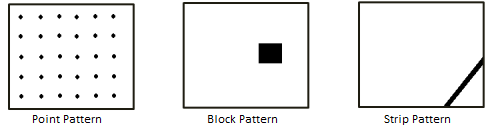
\includegraphics[width=8cm,height=2.5cm]{figures/ART_Patterns.png}
\caption{Failure patterns across input domain \cite{Chen2006}}
\label{fig:patterns}
\end{figure}

Chen et al. \cite{Chen2008} further found that there are patterns of failure causing inputs across the input domain. They divided these patterns into three types called block, point and strip patterns. They also argued that a strategy can get more chances of hitting these fault patterns if test cases far away from each other are selected. Various other researchers \cite{Chan2002}, \cite{Chen2003} and \cite{Chen2005} also tried to generate test cases further away from one another targeting these patterns and achieved higher performance. Failure patterns are illustrated in Figure \ref{fig:patterns}.\\


Random plus strategy \cite{Leitner2007} is an updated version of the pure random strategy. It is a modified form of random strategy that uses some special pre-defined values which can be simple border values or values that have high tendency of finding faults in the SUT. Boundary values \cite{Beizer1990} are the values on the start, end and middle of a particular type. For instance,  Integer.MIN\_VALUE -1, Integer.MIN\_VALUE, Integer.MIN\_VALUE +1, -3, -2, -1, 0, 1, 2, 3, Integer.MAX\_VALUE -1, Integer.MAX\_VALUE, Integer.MAX\_VALUE + 1, can be considered as border values for Integer data type. Similarly the tester might also add some other special values that he consider effective in finding faults for the current SUT. For example, if a program under test has a loop from 1 to 100 then the tester can add 100, 101, 99, 51, 50, 49, -1, 0 and 1 etc to the pre-defined list of special values in order to be selected for a test. This static list of interesting values is manually updated before the start of the test if require and has slightly high priority than selection of random values because of its more relevance and high chances of finding faults for the given SUT. It is found that these special values have high impact on the results particularly detecting problems in specifications \cite{Ciupa2008}.\\

The rest of this paper is organized as follows. The sections, II to X, describe Dirt Spot Sweeping Random (DSSR) strategy, Implementation of DSSR strategy, Experimental setup and analysis, Evaluation of DSSR strategy, Experimental results, Unique faults found by DSSR strategy, discussion, conclusion and future work respectively.\\ 